\documentclass[12pt,a4paper]{article}
\usepackage[utf8]{vietnam}
\usepackage{graphicx}
\usepackage{xcolor}
\usepackage{wrapfig}
\usepackage{multicol}
\usepackage{fancyhdr}
\usepackage{fancybox}
\usepackage[left=2.50cm, right=2.50cm, top=2.00cm, bottom=3.00cm]{geometry}
\pagestyle{fancy}
\fancyhf{}
\fancyhead[LE,RO]{\thepage}

\fancyhead[LO]{\small{\itshape{Lập trình PHP \& MySQL}}}
\begin{document}
\thispagestyle{empty}
\thisfancypage{
\setlength{\fboxsep}{0pt}
\fbox}{}
\begin{center}
\begin{large}
TRƯỜNG ĐẠI HỌC BÁCH KHOA HÀ NỘI
\end{large} \\
\begin{large}
VIỆN CÔNG NGHỆ THÔNG TIN VÀ TRUYỀN THÔNG
\end{large} \\

\textbf{--------------------  *  ---------------------}\\[1.5cm]

\includegraphics[scale=0.35]{12}
\\
\vspace{2cm}
{\fontsize{25pt}{1}\selectfont PROJECT I}\\[1cm]
{\fontsize{15pt}{1}\selectfont Lập trình Web}\\[1cm]
\end{center}
\hspace{3cm}
{\fontsize{12pt}{1}
\selectfont Sinh viên thưc hiện : } \hspace{1pt}
\textbf{\parbox[t]{6cm}{
\selectfont Nguyễn Quang Huy\\[0.3cm]
\selectfont MSSV : 20151690\\[0.3cm]
\selectfont Lớp : KSTN-CNTT-K60\\
   }
}\\[16pt]
\vspace{2cm}
\begin{center}
{\fontsize{12pt}{1}\selectfont HÀ NỘI}\\
{\fontsize{12pt}{1}\selectfont \today}
\end{center}
\newpage
\thispagestyle{empty}
\tableofcontents 
\newpage
\section{Hệ thống nhận dạng}
Hệ thống nhận dạng là một hệ thống tự động nhằm mục đích phân loại mẫu đầu vào thành một lớp cụ thể. Hệ thống tiến hành hai nhiệm vụ liên tiếp: (1) phân tích(hoặc mô tả) trích xuất đặc trưng từ mẫu đang được học và (2) phân lớp(hoặc nhận dạng) đối tượng sử dụng một số đặc trưng được trính xuất trong nhiệm vụ (1). \par 
Sơ đồ phân lớp dựa trên các mẫu đã được phân loại trong tập dữ liệu huấn luyện. Quá trình huấn luyện là quá trình học có giám sát, là thuật toán dự đoán đầu ra của một dữ liệu mới dựa trên các cặp đầu vào và nhãn lớp đã biết từ trước, phân lớp dựa trên các đặc tính của đối tượng. Phân tích mẫu cho phép sử dụng các đặc tính để mô tả và đại diện cho đối tượng thay vì tất cả các thuộc tính của đối tượng. \par 
\subsection{Sơ đồ khối hệ thống nhận dạng}
\begin{center}
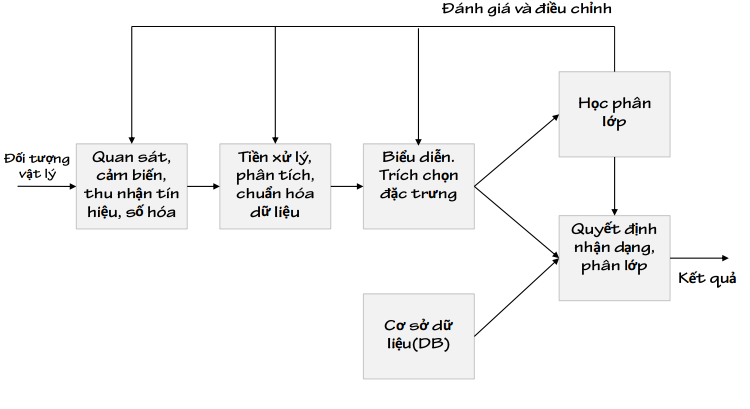
\includegraphics[scale=0.8]{23.png}\\
\textit{Sơ đồ chung của hệ thống nhận dạng}
\end{center}
\par 

Thiết kế cơ bản của một hệ thống nhận dạng liên quan đến 4 khía cạnh: 
\subsubsection{Thu thập dữ liệu}
Ảnh được chụp từ camera, qua quá trình số hóa ảnh(lấy mẫu tín hiệu và lượng tử hóa giá trị) thu được ảnh số. 
\subsubsection{Tiền xử lý ảnh}
Tiền xử lý ảnh nhằm mục đích lọc nhiễu, nâng cao chất lượng ảnh, chuẩn hóa kích cỡ ảnh. Nâng cao chất lượng ảnh làm cho ảnh tốt hơn theo ý đồ sử dụng. Đối với các ảnh thu được có nhiễu, cần loại bỏ nhiễu hay ảnh không sắc nét, ảnh bị mờ cần làm rõ các chi tiết. \par 
Ảnh với độ tương phản thấp có thể do không đủ điều kiện sáng, không đều, hoặc do tính không tuyến tính hay biến động nhỏ của bộ cảm nhận ảnh. Để điều chỉnh lại độ tương phản của ảnh, cần điều chỉnh lại biên độ trên toàn dải hay trên dải có giới hạn bằng cách biến đổi tuyến tính biên độ đầu vào. \par 
Tách nhiễu là trường hợp đặc biệt của dãn độ tương phản. Tách nhiễu được ứng dụng hiệu quả để giảm nhiễu khi biết tín hiệu vào trên khoảng xác định. Để làm trơn nhiễu hay tách nhiễu, sử dụng các bộ lọc tuyến tính(lọc trung bình, lọc thông thấp) hay lọc phi tuyến(trung vị, giả trung vị). \par 
Tách lấy vùng ảnh dữ liệu chứa đối tượng, hoặc tách lấy đối tượng cần nhận dạng trong ảnh, trừ nền, tách biệt ra khỏi các phần không liên quan đến đối tượng. 
\subsubsection{Biểu diễn, trích chọn đặc trưng}
Biểu diễn đối tượng dưới dạng các vector dữ liệu trong không gian nhiều chiều, mỗi chiều thể hiện cho một thuộc tính của đối tượng. Đối với ảnh, thuộc tính của đối tượng là các điểm ảnh, mỗi thuộc tính đối tượng có giá trị là giá trị của mỗi điểm ảnh. \par 
Trích chọn đặc trưng là phép biến đổi không gian biểu diễn dữ liệu đối tượng từ không gian quan sát(không gian dữ liệu ban đầu) sang không gian biểu diễn đặc trưng nhằm cho phép thực hiện hiệu quả quá trình học và ra quyết định phân lớp nhận dạng. 
\subsubsection{Học phân lớp}
Từ tập dữ liệu đã biểu diễn và trích chọn đặc trưng, với một số lượng dữ liệu đủ lớn, các đối tượng đã được gán nhãn ở bước biểu diễn và trích chọn đặc trưng, thực hiện quá trình phân lớp các đối tượng. Mỗi đối tượng sẽ có một tập các vector dữ liệu biểu diễn đối tượng đó ở các trạng thái khác nhau, các trạng thái này có được trong quá trình thu thập dữ liệu. \par 
Mục đích của quá trình học phân lớp là xây dựng hàm phân lớp từ dữ liệu huấn luyện. 
\subsubsection{Quyết định nhận dạng, phân lớp}
Sau khi đã có được hàm phân lớp từ quá trình học phân lớp, thực hiện tính toán với dữ liệu đưa vào cần nhận dạng theo hàm phân lớp tìm được, đưa ra quyết định nhận dạng, phân lớp đối tượng. 

\subsection{Vai trò của SVM trong hệ thống nhận dạng}
Support Vector Machine là một thuật toán học có giám sát, đóng vai trò học phân lớp và quyết định nhận dạng đối tượng trong hệ thống nhận dạng. Trong hệ thống nhận dạng, SVM sử dụng dữ liệu huấn luyện có được từ bước biểu diễn và trích chọn đặc trưng làm đầu vào, mỗi đối tượng khác nhau đóng vai trò là một lớp, thực hiện tìm các mặt siêu phẳng phân cách các lớp trong không gian nhiều chiều. Để đưa ra quyết định nhận dạng, bản chất SVM là tìm ra các hàm phân lớp tuyến tính các đối tượng, sử dụng hàm phân lớp tìm được trong quá trình huấn luyện để đưa ra kết quả với đầu vào là dữ liệu đối tượng cần nhận dạng. 
\section{Hệ thống nhận dạng khuôn mặt sử dụng SVM}
Từ sơ đồ chung của một hệ thống nhận dạng, hệ thống nhận dạng khuôn mặt sử dụng SVM bao gồm hai quá trình:
\begin{center}

\includegraphics[scale=0.6]{25.png}\\
\textit{Sơ đồ khối hệ thống nhận dạng khuôn mặt sử dụng SVM}
\end{center}  
\par 
Sau quá trình quan sát cảm biến, thu nhận tín hiệu, số hóa thu được ảnh số. Hệ thống thực hiện tiền xử lý, phân tích, chuẩn hóa dữ liệu. Ở bước này, thực hiện lọc nhiễu, nâng cao chất lượng ảnh, chuẩn hóa kích thước ảnh. Đối với ảnh chứa khuôn mặt, hệ thống phát hiện và phân tách khuôn mặt và lấy vùng ảnh chứa khuôn mặt. Bước tiếp theo, biểu diễn ảnh thu được dưới dạng vector trong tọa độ không gian nhiều chiều, mỗi chiều biểu diễn một thuộc tính có giá trị là giá trị điểm ảnh tương ứng, vector này có được từ phép chuyển đổi ma trận dữ liệu ảnh tương ứng. \par    
\subsection{Huấn luyện}
Đầu vào của quá trình huấn luyện là tập dữ liệu các đối tượng đã được gán nhãn. Sau khi có tập dữ liệu được biểu diễn dưới dạng các vector, tiến hành trích chọn đặc trưng, biến đổi không gian biểu diễn dữ liệu đối tượng từ không gian quan sát sang không gian biểu diễn đặc trưng. Trong hệ thống nhận dạng khuôn mặt này, sử dụng phép biến đổi \textbf{PCA} để thực hiện trích chọn đặc trưng. Phép biến đổi \textbf{PCA} thực hiện trích chọn ra và giữ lại \textit{k} thành phần khác nhau nhất giữa các vector dữ liệu phục vụ hiệu quả cho quá trình học và ra quyết định phân lớp nhận dạng. Đầu vào của quá trình huấn luyện là các vector dữ liệu \textit{k} thành phần thu được từ phép biến đổi \textbf{PCA}, \textit{k} thành phần cũng là \textit{k} thuộc tính của các đối tượng dùng để đối sánh và phân lớp. Mỗi đối tượng được gán nhãn các lớp tương ứng, các vector biểu diễn cùng một đối tượng có cùng nhãn, ngược lại, các vector biểu diễn các đối tượng khác nhau có nhãn khác nhau. Bước tiếp theo tiến hành phân lớp đối tượng sử dụng \textbf{SVM}, tìm ra các mặt phân cách giữa các lớp và hàm phân tách tuyến tính các lớp. Lưu lại hàm phân lớp tìm được và ma trận phép biến đổi \textbf{PCA} trong cơ sở dữ liệu, làm cơ sở cho quá trình quyết định nhận dạng. 
\subsection{Quyết định nhận dạng} 
Đầu vào của quá trình quyết định nhận dạng là dữ liệu đối tượng cần nhận dạng. Từ ảnh chứa đối tượng cần nhận dạng, thực hiện bước tiền xử lý và biểu diễn đối tượng dưới dạng vector dữ liệu trong không gian(đây là giai đoạn chung của cả hệ thống, sử dụng cho cả quá trình huấn luyện và quá trình nhận dạng). Sau khi biểu diễn đối tượng cần nhận dạng, thực hiện phép biến đổi \textbf{PCA} để trích chọn đặc trưng, giảm số chiều của vector dữ liệu, giữ lại \textit{k} thành phần của đối tượng, sử dụng ma trận phép biến đổi \textbf{PCA} có được từ quá trình huấn luyện, được lưu trữ trong cơ sở dữ liệu, thu được vector dữ liệu \textit{k} thành phần biểu diễn \textit{k} thuộc tính của đối tượng cần nhận dạng.
Sử dụng hàm phân lớp tìm được từ quá trình huấn luyện, được lưu trữ trong cơ sở dữ liệu, đầu vào là vector dữ liệu đã thu được, quyết định nhận dạng đối tượng và đưa ra kết quả. 

\section{Cài đặt thử nghiệm}
Các bước thực hiện: 
\begin{itemize}
\item Thu thập tín hiệu, số hóa 
\begin{itemize}
\item Thực hiện thu thập 201 ảnh của 5 người khác nhau. Mỗi người với số lượng ảnh lần lượt là 31, 56, 39, 61 và 14 ảnh. 
\end{itemize}
\end{itemize}    

      
\newpage
\section{Tài liệu tham khảo}
\begin{enumerate}
\item http://tuanduongcntt.blogspot.com/2014/05/lap-trinh-php-co-ban-giao-trinh-fpt.html
\item https://sites.google.com/site/khaiphongphp/slidebaigiang
\item https://www.w3schools.com/php
\item https://www.w3schools.com/html
\item https://www.w3schools.com/css
\item https://www.w3schools.com/js
\item https://jquery.com
\item http://php.net/
\item Lập trình PHP Khoa Phạm
\end{enumerate}    
\end{document}